\documentclass[10pt]{article}
\usepackage[margin=0.85in]{geometry}
\usepackage{amsmath,amssymb,amsthm}
\usepackage{graphicx}
\usepackage{caption}
\usepackage{kotex}
\captionsetup{font=small}

\newtheorem{proposition}{Proposition}

\newcommand{\supIPM}{\mathrm{supIPM}}
\newcommand{\EIPM}{\mathrm{EIPM}}
\newcommand{\hsupIPM}{\widehat{\supIPM}}
\newcommand{\Wone}{W_1}

\pagestyle{empty}
\begin{document}

\begin{center}\vspace{-0.5em}
{\large\bfseries Experiment}
\vspace{-0.5em}\end{center}


\section{Simulation}

\paragraph{Purpose.} Two things. \emph{(1)} The motivation for using the supremum. \emph{(2)} Our estimator $\hsupIPM$ recovers the true
$\supIPM$.

\begin{itemize}
    \item 지금은 discriminator가 holder space여서 IPM이 closed form으로 나오는 경우로 해놨는데 이걸 똑같이 relu discriminator로 바꾸는게 맞지 않을까?? 라는 생각
\end{itemize}

\begin{proposition}
For a joint law $P$ of $(S,Z)$ with $S$ absolutely continuous, let
$\Delta_P(s) = \sup_{f \in \mathrm{Lip}_1} \big| \mathbb E_P[f(Z) \mid S{=}s] - \mathbb E_P[f(Z)] \big|$.
For every $\varepsilon, M > 0$ there is such a $P$, with $S \sim N(0,1)$ and
$\operatorname{Var}_P(Z) = 1$, satisfying
\[
\mathbb E_P\big[\Delta_P(S)\big] \;\le\; \varepsilon
\qquad\text{and}\qquad
\operatorname*{sup}_{s} \Delta_P(s) \;\ge\; M .
\]
\end{proposition}

\noindent The converse inequality is trivial, so $\supIPM$ is a strictly stronger guarantee.


\paragraph{Data.}
\[
S \sim N(0,1), \qquad Z \mid S{=}s \sim N\!\big(\mu(s),\,\sigma_c^2\big),
\qquad \mu(s) = \kappa\exp\!\Big(\!-\tfrac{(s-s_0)^2}{2\tau^2}\Big),
\qquad \kappa = 1.2,\ \ s_0 = 0.7,\ \ \tau = 0.2,
\]
with $\sigma_c^2 = 1 - \operatorname{Var}(\mu(S))$ so that $\operatorname{Var}(Z) = 1$. 

\paragraph{Estimator.} For a fixed $s$, weight each observation by how close $s_i$ is to $s$, and
compare the resulting conditional distribution to the pooled one:
\[
\widehat F_s(u) = \sum_i w_i(s)\,\mathbf 1(z_i \le u), \qquad
w_i(s) = \frac{K_h(s-s_i)}{\sum_j K_h(s-s_j)}, \qquad
\widehat \Wone(s) = \int \big|\widehat F_s(u) - \widehat F(u)\big|\,du ,
\]
with $K_h$ a Gaussian kernel of bandwidth $h$ and $\widehat F$ the pooled empirical CDF. 
We use $h = 0.25\,n^{-1/5}$, grid spacing $h/2$, and $n = 500,\dots,2{\times}10^4$ with $100$
replications each.

\paragraph{Why this design.} With a $\mathrm{Lip}_1$ discriminator $\mathrm{IPM} = \Wone$, and for
one-dimensional $Z$ the truth is available in closed form, so the estimator can be checked against
it. This setting makes $\supIPM$ large while $\EIPM$ stays small.



% \paragraph{What we measure.} The estimated curve $\widehat \Wone(\cdot)$ against the truth, and the
% error of $\hsupIPM$ against the rate $n^{-2/5}$. The curve matters because
% $|\max_s \widehat \Wone - \max_s \Wone| \le \|\widehat \Wone - \Wone\|_\infty$ --- a supremum is
% reliable only if the estimate is close everywhere.

\paragraph{Result.} 
The followings are result.
\begin{figure}[!h]\vspace{-0.5em}
\centering
    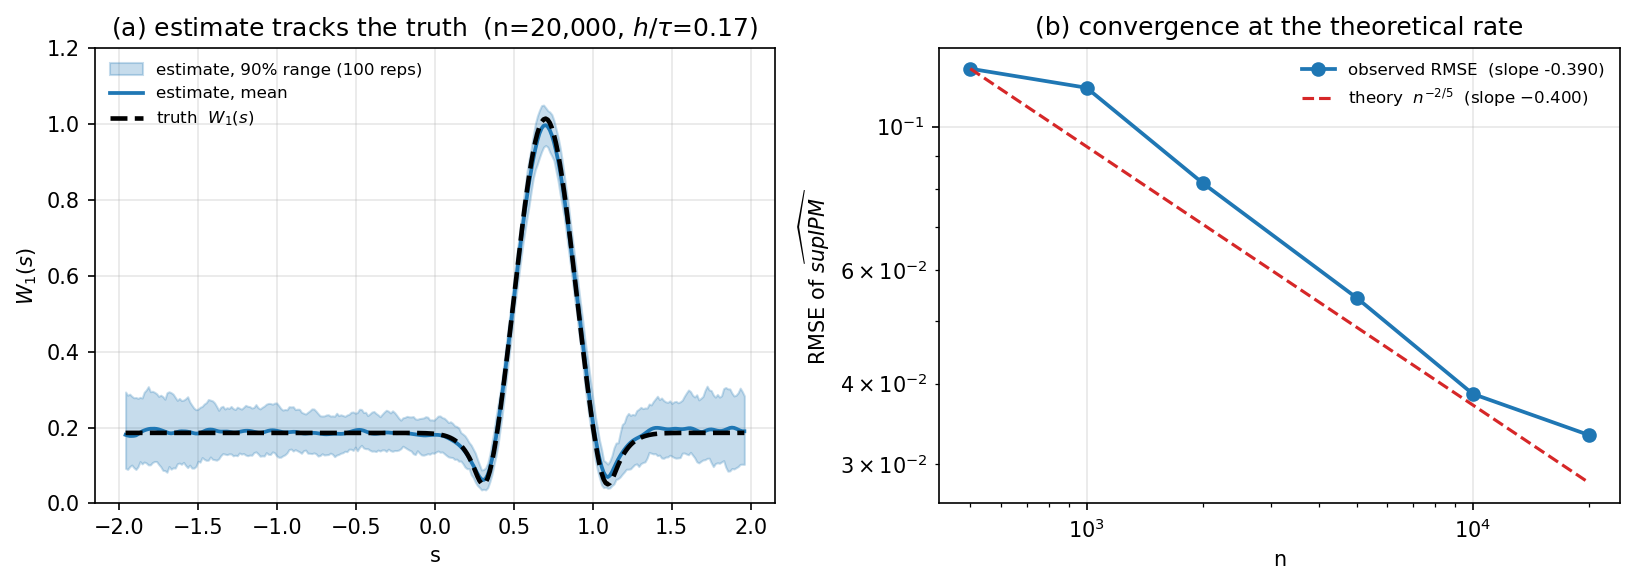
\includegraphics[width=1\linewidth]{figures//Simulation/S1_main.png}
\caption{(a) $\widehat{W_1}(s)$ against the truth
($n = 2{\times}10^4$). (b) RMSE of $\hsupIPM$ vs.\ $n$, with the theoretical
$n^{-2/5}$ line.}
\end{figure}
\vspace{-0.5em}


% \paragraph{Result.} The estimate tracks the truth uniformly in $s$, recovers both the peak and its
% location, and converges at the theoretical rate. The bandwidth must stay below the bump width $\tau$
% for this to hold: a wider kernel averages over a window larger than the bump, flattening the peak, and
% the rate is not attained --- as expected, since the expansion $\mathrm{bias} = O(h^2)$ presumes
% $h < \tau$. The resulting bias is always negative, so an oversized bandwidth reports the
% representation as \emph{fairer} than it is. Since $\tau$ is unknown in real data, how to choose $h$
% remains open.


\newpage

\section{Main}

\subsection{ReLU-IPM}

\begin{itemize}
    \item 다음과 같은 discriminator class $\mathcal{F}_{\mathbf{ReLU}}$를 생각하자.
    \begin{equation*}
        \mathcal{F}_{\mathbf{ReLU}} := \{f: \mathbb{B}^{d} \rightarrow \mathbb{R} | f(\mathbf{z}) = (\theta^{\top} \mathbf{z} + \mu)_{+},\, \mu \in [-1,1], \, \theta \in \mathbb{S}^{d-1}\}
        ,
    \end{equation*}
    where $\mathbb{S}^{d-1} = \{\mathbf{z} \in \mathbb{R}^{d} : || \mathbf{z} ||_{2} =1 \}$.
    \item Input $\mathbf{X} \in \mathcal{X}$와 output $Y$가 있고, encoder $h_{\phi}: \mathcal{X} \rightarrow \mathbb{R}^{d}$ 그리고 head는 $f_{\psi}$가 주어졌다 하자.
    \item 이 때, $\mathbf{Z} = h_{\phi}(\mathbf{X})$ 이고, $\tilde{\mathbf{Z}}  = \frac{\mathbf{Z}}{\sqrt{||\mathbf{Z}||^{2} + 1}}$로 정의한다.
    \item 이 때, 우리가 원하는 것은 continuous sensitive attribute $S$에 대해서 $\tilde{\mathbf{Z}}$의 분포와 $\tilde{\mathbf{Z}} |S$의 분포가 IPM 측면에서 가까워지는 것이다.
    \item 즉, 
    \begin{equation*}
        \mathrm{IPM}_{\mathcal{V}}(\mathbb{P}_{\tilde{\mathbf{Z}} |S} , \mathbb{P}_{\tilde{\mathbf{Z}}})
    \end{equation*}
    를 작게 만들고자 한다.
    \item 이때, $\mathcal{V} = \mathcal{F}_{\mathbf{ReLU}}$를 사용하고, $S$에 대해 평균이 아닌, 상한을 취해서 SupIPM을 정의한다.
    \begin{equation*}
    \begin{aligned}
        \mathrm{SupIPM}_{\mathcal{F}_{\mathbf{ReLU}}} (\mathbf{Z} ; S) :&= \sup_{S} [\mathrm{IPM}_{ \mathcal{F}_{\mathbf{ReLU}}}(\mathbb{P}_{\tilde{\mathbf{Z}} |S} , \mathbb{P}_{\tilde{\mathbf{Z}}})] \\
        &=\sup_{S} \sup_{v \in  \mathcal{F}_{\mathbf{ReLU}}} |\mathbb{E}_{\tilde{\mathbf{Z}} |S}v(\tilde{\mathbf{Z}})-         \mathbb{E}_{\tilde{\mathbf{Z}}}v(\tilde{\mathbf{Z}})| \\
        &=\sup_{S} \sup_{v \in  \mathcal{F}_{\mathbf{ReLU}}} | \int v(\tilde{\mathbf{z}}) (d\mathbb{P}_{\tilde{\mathbf{Z}} |S}(\tilde{\mathbf{z}}) - d\mathbb{P}_{\tilde{\mathbf{Z}}}(\tilde{\mathbf{z}})) |
    \end{aligned}
    \end{equation*}
    \item 이제, 데이터 $\mathcal{D} = \{(x_i, s_i, y_i)\}_{i=1}^{n}$이 주어졌다 하자. 이 데이터를 사용해서 $\mathbb{P}_{\tilde{\mathbf{Z}} |S} $을 추정해야 하지만 $S=s$에 속한 원소가 두개 이상이 될 수가 없어서 일반적인 empirical distribution으로 추정이 불가능하다. 그렇기 때문에 kernel을 사용한다. FREM에서 제안한 바를 따라서, $\widehat{\mathbb{P}}_{\tilde{\mathbf{Z}} |S} $를 다음과 같이 구한다.
    \begin{equation*}
        \widehat{\mathbb{P}}_{\tilde{\mathbf{Z}} |S=s} = \sum_{i=1}^{n} \frac{K_{h}(s, s_i)}{\sum_{j} K_{h}(s,s_j)} \delta_{\mathbf{\tilde{Z}_{i}}} 
    \end{equation*}
    \item 이를 사용해, $\mathrm{SupIPM}_{\mathcal{F}_{\mathbf{ReLU}}} (\mathbf{\tilde{Z}} ; S)$를 다음과 같이 추정한다.
    \begin{equation*}
        \widehat{\mathrm{SupIPM}}_{\mathcal{F}_{\mathbf{ReLU}}} (\mathbf{\tilde{Z}} ; S)  =  \sup_{S} \sup_{v \in  \mathcal{F}_{\mathbf{ReLU}}} |\sum_{i=1}^{n} \left(w_i(s) - \frac{1}{n} \right) v(\tilde{\mathbf{z}_i}) |
    \end{equation*}
    이 때, $w_i(s) =  \frac{K_{h}(s, s_i)}{\sum_{j} K_{h}(s,s_j)}$이다.
\end{itemize}

\subsection{Objective function}
\begin{itemize}
    \item 이 때, 최적화하는 objective function은 다음과 같다.
    \begin{equation*}
        \mathcal{L}(\phi, \psi) = \frac{1}{n} \sum_{i=1}^{n} l(f_\psi(\tilde{\mathbf{z}}_i), y_i) + \lambda \widehat{\mathrm{SupIPM}}_{\mathcal{F}_{\mathbf{ReLU}}} (\mathbf{\tilde{Z}} ; S) 
    \end{equation*}
\end{itemize}


\subsection{Algorithm}
\begin{itemize}
    \item $ \widehat{\mathrm{SupIPM}}_{\mathcal{F}_{\mathbf{ReLU}}}$의 계산은 ReLU-IPM의 알고리즘을 변형해서 할 수 있다.
    
    \item Encoder $h_{\phi}$가 주어져 있다고 하자. 그러면 $\tilde{\mathbf{z}}_i$는 바로 계산 가능하다. 이 때 $c=1,\cdots,K$에 대해서 $v_{c} = (\mu_c, \theta_c)$를 초기화시킨다 (실험에선 $K=100$ 사용). 그리고 $\mathbf{v} = (v_1,\cdots, v_K)^{\top}$라 하자.
    \item 마찬가지로 $s^{(t)}, t=1,\cdots, T$를 초기화시킨다 (실험에서는 $T=8$ 사용). 마찬가지로 $\mathbf{s} = (s^{(1)}, \cdots, s^{(T)})^{\top}$라 하자.
    \item 이때 표기의 편의를 위해서,
    \begin{equation*}
        \Delta_{c}(s) =  |\sum_{i=1}^{n} \left(w_i(s) - \frac{1}{n} \right) 
        v_c(\tilde{\mathbf{z}_i}) |, \quad v_c(\tilde{\mathbf{z}}) = (\theta_{c}^{\top}\tilde{\mathbf{z}} + \mu )_{+}
    \end{equation*}
    라 하자.
    \item 이 때 $(\Delta_{c}(s^{(t)}))_{t,c} \in \mathbb{R}^{T \times K}$이고, 여기서 rowwise maximum을 한것의 합을 $g(\mathbf{s})$라 정의하자. 즉,
    \begin{equation*}
        g(\mathbf{s}) = \sum_{t=1}^{T} \max_{c=1,\cdots K}  \Delta_{c}( s^{(t)} ).
    \end{equation*}
    그리고 나서 $\mathbf{s} \leftarrow \mathbf{s} + \nu \nabla_{\mathbf{s}} g(\mathbf{s})$로 20 step 업데이트해서 gradient ascent한다.
    \item 그 뒤 $s^{\star}$를 다음과 같이 정의한다.
    \begin{equation*}
        s^{\star} = \mathrm{argmax}_{s^{(t)}}  \max_{c=1,\cdots K}  \Delta_{c}( s^{(t)} ) 
    \end{equation*}
    \item 이제 이 $s^{\star}$를 사용해서 discriminator를 update 한다.
    \item 이 역시 $h(\mathbf{v})$역시 다음과 같이 정의한다.
    \begin{equation*}
        h(\mathbf{v}) = \sum_{c=1}^{K} \Delta_{c}(s^{\star})
    \end{equation*}
    \item 이를 사용해 $\mathbf{v} \leftarrow \mathbf{v} + \eta \nabla_{\mathbf{v}} h(\mathbf{v})$로 1 step update 한다.
    \item 이렇게 $s^\star$를 찾고 $\mathbf{v}$ 업데이트 하는 과정을 critic step (기본은 2번) 반복한다. 그 뒤 마지막으로 $s^\star$를 찾는다.
    \item 이렇게 구한 $s^\star$와 $\mathbf{v}$를 목적함수에 대입하여 $\phi$와 $\psi$를 최적화한다.
    \item 그렇게 구한 enconder, head로 다시  $s^\star$와 $\mathbf{v}$를 최적화한다.
    \item 이것을 전체 epoch (기본 200회)만큼 반복한다.
\end{itemize}

\section{Problem}
\begin{itemize}
    \item 지금 실제로 문제가 되는 부분은 2가지가 있다.
    \item 실제 코드를 구현할 때 S의 domain의 양극단은 잘라내고 안쪽에서만 s를 최적화 시킴. $s$가 극단에 있을시에 조건부분포가 점분포가 될수있어서.
    \item 지금 처럼 구현할수에 critic step이 2번일시에 수렴하지 않음. 20번 이상 반복해야 수렴하는데 이럴 시 계산량이 너무 많아지는 문제.
\end{itemize}
\end{document}